\section[Delegation]{From asking questions to delegating work}
\sectionframe{01}{From asking questions to delegating work}
  {What must we provide, and what must we verify, before an agent takes over a task?}
  {\faRobot}

% ---------------------------------------------------------- chat vs agent
\begin{frame}{From a chat assistant to a coding agent}
  \begin{tikzpicture}[x=1mm,y=1mm,
      who/.style={minimum width=15mm,minimum height=9.5mm,font=\small\bfseries}]
    % conversational assistant
    \node[anchor=north west,inner sep=0pt,font=\small\bfseries] at (0,0) {Conversational assistant};
    \node[anchor=north west,lbl,inner sep=0pt,font=\footnotesize] at (0,-4.6) {answers questions about what you paste};
    \node[human,who] (you1) at (8,-25.25) {You};
    \node[agent,who] (llm) at (56,-25.25) {Model};
    \draw[flow] ([yshift=2.2mm]you1.east) -- node[lbl,above]{question, pasted code} ([yshift=2.2mm]llm.west);
    \draw[flow] ([yshift=-2.2mm]llm.west) -- node[lbl,below]{answer, snippet} ([yshift=-2.2mm]you1.east);
    \node[anchor=north west,text width=64mm,font=\footnotesize,inner sep=0pt] at (0,-46)
      {you run the code; it sees only what you paste};
    \draw[udsgreylight,line width=0.4pt] (67,0) -- (67,-51);
    % coding agent
    \node[anchor=north west,inner sep=0pt,font=\small\bfseries] at (72,0) {Coding agent};
    \node[anchor=north west,lbl,inner sep=0pt,font=\footnotesize] at (72,-4.6) {acts in your repository};
    \node[human,who] (you2) at (79.5,-25.25) {You};
    \draw[udsblue,dashed,line width=0.5pt] (101,-10) rectangle (143.4,-40.5);
    \node[anchor=south east,lbl,text=udsblue] at (143.4,-9.8) {sandbox: repository, shell, approvals};
    \coordinate (c) at (122.2,-25.25);
    \foreach \a/\t in {90/read files,0/edit,270/run tests,180/inspect} {
      \node[agent,inner sep=1mm,font=\footnotesize] (n\a) at ($(c)+(\a:12.5 and 9.6)$) {\t};
    }
    \draw[flow,draw=udsblue] (n90.east) to[bend left=30] (n0.north);
    \draw[flow,draw=udsblue] (n0.south) to[bend left=30] (n270.east);
    \draw[flow,draw=udsblue] (n270.west) to[bend left=30] (n180.south);
    \draw[flow,draw=udsblue] (n180.north) to[bend left=30] (n90.west);
    \draw[flow] ([yshift=2.2mm]you2.east) -- node[lbl,above]{task} ([yshift=2.2mm]you2.east -| 101,0);
    \draw[flow] ([yshift=-2.2mm]you2.east -| 101,0) -- node[lbl,below]{diff, report} ([yshift=-2.2mm]you2.east);
    \node[anchor=north west,text width=71mm,font=\footnotesize,inner sep=0pt] at (72,-46)
      {loops until done; you set limits, accept or reject};
  \end{tikzpicture}
  \note{\textbf{1:10--2:20}\par
    A chat assistant answers questions; we stay the integrator and carry code and results back
      and forth.\par
    An agent has tools: it reads the repository, edits files, runs commands and iterates until
      it judges the task done.\par
    That makes delegation possible, but it works with whatever context and permissions we give
      it.\par
    Those permissions are its sandbox: the folders it may change, the commands it may run, and
      what it must ask us first.\par
    Its typical failure is not a syntax error but a reasonable-looking change that violates
      something only we know, such as how the data must be split.}
\end{frame}

% -------------------------------------------------------- running example
\begin{frame}{Running example: split the data by specimen}
  % oblique view: a point (p,q) of a micrograph lying flat goes to (p + \obs q, \obk q)
  \def\obs{0.5}\def\obk{0.42}
  \def\ow{34}\def\oh{24.51}% overview micrographs, 1000 x 721 px
  \def\dw{28}\def\dh{20.02}% detail micrographs, 1000 x 715 px
  \begin{tikzpicture}[x=1mm,y=1mm,
      sheet/.style={draw=udsdark,line width=0.35pt},
      tag/.style={anchor=south west,fill=udsdark,fill opacity=0.8,text opacity=1,text=white,
        font=\ttfamily\fontsize{7}{8}\selectfont,inner xsep=0.8mm,inner ysep=0.4mm},
      zoom/.style={udsblue,line width=0.4pt},
      side/.style={anchor=west,font=\scriptsize,inner sep=0pt}]
    % ---------------------------------------------------------------- specimens
    \node[anchor=north west,inner sep=0pt,font=\footnotesize] at (0,0) {\textbf{Specimens}\enspace one per state};
    \foreach \n [count=\i] in {AsCast,Q980\_0h\_WC,Q980\_9h\_AC} {
      \begin{scope}[shift={(18,{-10-(\i-1)*11})}]
        \fill[udsgreylight] (0,0) rectangle (12,-2);
        \fill[udsgreymid] (12,0) -- (16,3.36) -- (16,1.36) -- (12,-2) -- cycle;
        \fill[udsgreypale] (0,0) -- (12,0) -- (16,3.36) -- (4,3.36) -- cycle;
      \end{scope}
      \node[anchor=east,inner sep=0pt,font=\ttfamily\fontsize{7}{8}\selectfont] at (16.5,{-9.2-(\i-1)*11}) {\n};
      \node[anchor=east,inner sep=0pt,font=\scriptsize,text=udsgrey] at (16.5,{-12.4-(\i-1)*11}) {fold \i};
    }
    % the specimen of the running example; a tiny copy of its overview micrograph marks the imaged
    % spot (not to scale)
    \draw[udsblue,line width=0.8pt] (18,-21) -- (30,-21) -- (34,-17.64) -- (22,-17.64) -- cycle;
    \begin{scope}[cm={1,0,\obs,\obk,(18,-21)}]
      \node[anchor=south west,inner sep=0pt,transform shape] at (4.3,2.78)
        {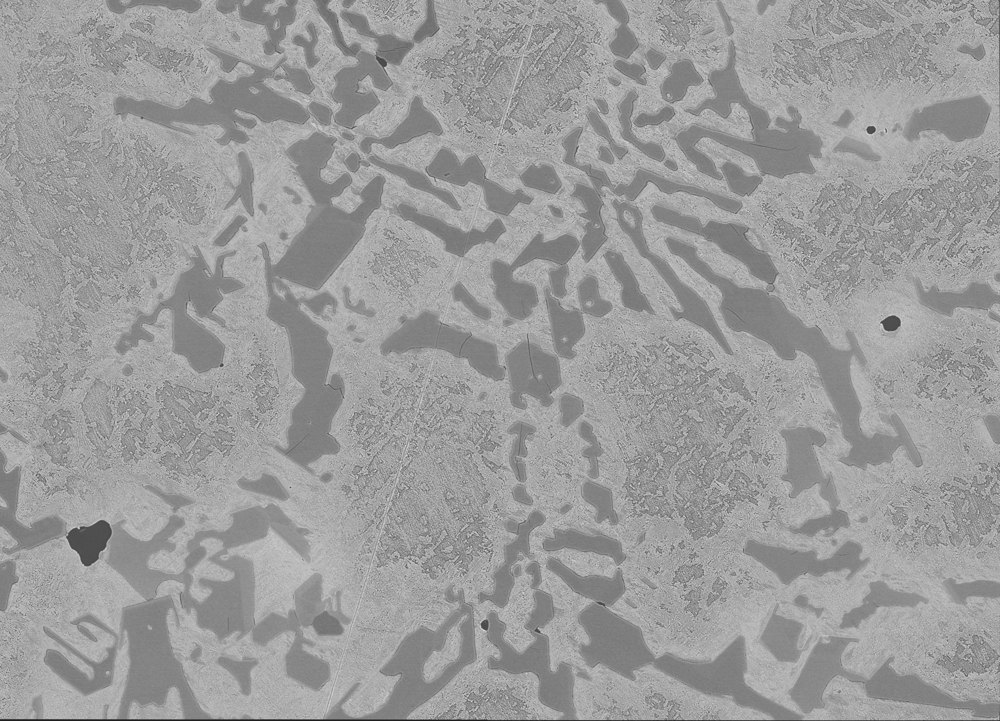
\includegraphics[width=3.4mm,height=2.45mm]{assets/hcci/overview-bse}};
      \draw[udsblue,line width=0.6pt] (4.3,2.78) rectangle (7.7,5.23);
      \coordinate (sa) at (7.7,5.23); \coordinate (sb) at (4.3,2.78);
    \end{scope}
    % ------------------------------------------------------------ overview area
    \node[anchor=north west,inner sep=0pt,font=\footnotesize,align=left] at (38,-10)
      {\textbf{Overview area}\\[0.3mm]{\scriptsize\color{udsgrey}66 micrographs on one pixel grid}};
    \draw[zoom] (sa) -- (38+\obs*\oh,-30+\obk*\oh) (sb) -- (38,-30);
    \foreach \img/\y in {overview-inlens/-32.8,overview-se/-31.4,overview-bse/-30} {
      \begin{scope}[cm={1,0,\obs,\obk,(38,\y)}]
        \node[anchor=south west,inner sep=0pt,transform shape] at (0,0)
          {\includegraphics[width=\ow mm,height=\oh mm]{assets/hcci/\img}};
        \draw[sheet] (0,0) rectangle (\ow,\oh);
      \end{scope}
    }
    % the detail area inside it, where the dataset README places it (section 7)
    \begin{scope}[cm={1,0,\obs,\obk,(38,-30)}]
      \draw[udsblue,line width=0.8pt] (0.6071*\ow,0.4589*\oh) rectangle (0.7999*\ow,0.6500*\oh);
      \coordinate (f1) at (0.6071*\ow,0.4589*\oh); \coordinate (f2) at (0.7999*\ow,0.4589*\oh);
      \coordinate (f3) at (0.7999*\ow,0.6500*\oh);
    \end{scope}
    % -------------------------------------------------------------- detail area
    \node[anchor=north west,inner sep=0pt,font=\footnotesize,align=left] at (89,0)
      {\textbf{Detail area}\enspace inside it, 5$\times$ finer\\[0.3mm]{\scriptsize\color{udsgrey}60 micrographs on one pixel grid}};
    % from the box's lower-left, lower-right and upper-right corners to the near corner of each
    % micrograph, so no line crosses the box
    \draw[zoom] (f1) -- (89,-40) (f2) -- (89,-32.8) (f3) -- (89,-25.6);
    % more micrographs under the stack: other microscopes, voltages and dwell times
    \foreach \y in {-42.8,-41.4} {
      \begin{scope}[cm={1,0,\obs,\obk,(89,\y)}]
        \filldraw[fill=udsgreypale,sheet] (0,0) rectangle (\dw,\dh);
      \end{scope}
    }
    % the patch: the same pixels in every micrograph of the area
    \def\pa{0.42*\dw}\def\pb{0.67*\dw}\def\pc{0.25*\dh}\def\pd{0.58*\dh}
    \foreach \img/\y/\col/\detector/\role in {detail-bse/-40/udsblue/BSE/training,
        detail-se/-32.8/udsred/SE/validation,detail-inlens/-25.6/udsblue/InLens/training} {
      \begin{scope}[cm={1,0,\obs,\obk,(89,\y)}]
        \node[anchor=south west,inner sep=0pt,transform shape] at (0,0)
          {\includegraphics[width=\dw mm,height=\dh mm]{assets/hcci/\img}};
        \draw[sheet] (0,0) rectangle (\dw,\dh);
        \fill[\col,fill opacity=0.35] (\pa,\pc) rectangle (\pb,\pd);
        \draw[\col,line width=0.9pt] (\pa,\pc) rectangle (\pb,\pd);
      \end{scope}
      \node[tag] at (89.5,\y+0.5) {\detector};
      \node[side,text=\col] at (129,\y+4) {\role};
      % the column up to the next sheet, which hides the part beneath it
      \foreach \p/\q in {\pa/\pc,\pb/\pc,\pa/\pd,\pb/\pd}
        \draw[udsdark,line width=0.35pt,dash pattern=on 0.8pt off 0.6pt]
          (89+\p+\obs*\q,\y+\obk*\q) -- ++(0,7.2);
    }
    \begin{scope}[cm={1,0,\obs,\obk,(89,-18.4)}]
      \node[anchor=south west,inner sep=0pt,transform shape] at (0,0)
        {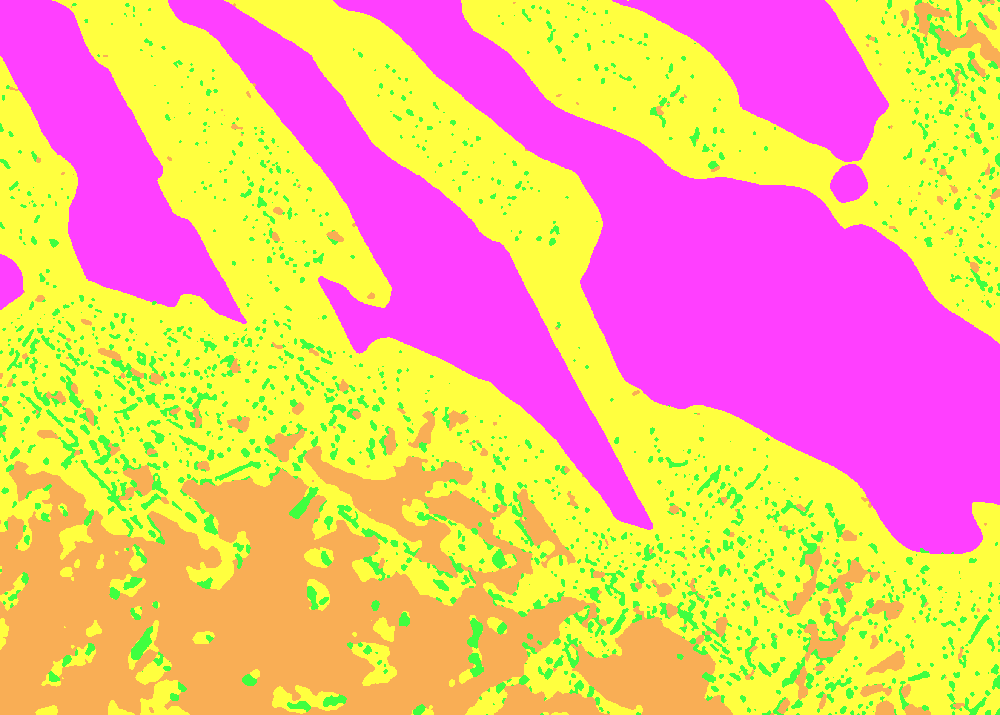
\includegraphics[width=\dw mm,height=\dh mm]{assets/hcci/detail-mask}};
      \draw[sheet] (0,0) rectangle (\dw,\dh);
      \draw[udsdark,line width=0.9pt] (\pa,\pc) rectangle (\pb,\pd);
    \end{scope}
    \node[side,text=udsdark] at (129,-14.4) {one mask};
    % ------------------------------------------------------------------- result
    \node[anchor=north west,inner sep=0pt,font=\footnotesize,text=udsred] at (38,-44.5)
      {\textbf{Random patch split}\enspace one area, one mask on both sides: data leakage};
    \node[anchor=north west,inner sep=0pt,font=\footnotesize] at (0,-50.5)
      {\textbf{Task}\enspace validation folds by specimen, every specimen in exactly one fold};
  \end{tikzpicture}
  \note{\textbf{2:20--3:40}\par
    The running example uses our HCCI dataset: one specimen per material state.\par
    On each specimen one overview area was imaged, and a detail area inside it at five times
      finer sampling.\par
    Every area was imaged about 60 times: four microscopes, two or three detectors, three
      voltages, two dwell times.\par
    All micrographs of an area sit on one pixel grid and share one mask, annotated once by
      hand.\par
    The model trains on patches, crops of these micrographs.\par
    A random split can put this patch of the SE micrograph in validation and the same pixels of
      the BSE and in-lens micrographs in training.\par
    The model has then seen this area and its mask, so the validation score rewards recognising
      it: that is data leakage.\par
    The detail area and the second etching overlap too; only the specimens share nothing.\par
    So the task is validation folds by specimen, every specimen in exactly one fold.}
\end{frame}

% ----------------------------------------------------------- weak request
\begin{frame}{A weak request}
  \begin{tikzpicture}[x=1mm,y=1mm]
    % the cards fill the text width exactly; strokes on their edges must not widen the picture
    \useasboundingbox (0,0) rectangle (144,-54);
    \specterminal{0}{the request}
    % each vague phrase is a node of its own, so an arrow can leave from it
    \node[spec request] (r0) at (term) {>\specspace};
    \node[spec request] (p1) at (r0.base east) {Update the dataset code};
    \node[spec request] (r1) at (p1.base east) {\specspace so we split our SEM data\specspace};
    \node[spec request] (p2) at (r1.base east) {by sample};
    \node[spec request] (r2) at (p2.base east) {\specspace instead of randomly, and\specspace};
    \node[spec request] (p3) at (r2.base east) {add a test};
    \node[spec request] at (p3.base east) {.};
    \foreach \p in {p1,p2,p3}
      \draw[termred,line width=0.8pt] ([yshift=-1.1mm]\p.base west) -- ([yshift=-1.1mm]\p.base east);
    % the five parts; dashed: not in the request at all
    \foreach \k/\l/\f in {0/Objective/bluetint,1/Context/bluetint,2/Constraints/white,
        3/Acceptance/bluetint,4/Verification/white}
      {\speccard{\k}{-24}{-50.6}{\l}{\f}}
    \foreach \k in {2,4} {
      \draw[udsgreymid,dashed,line width=0.6pt] (\k*28.9,-29.4) rectangle (\k*28.9+28.4,-50.6);
      \node[anchor=south west,inner sep=0pt,font=\scriptsize\itshape,text=udsred] at (\k*28.9+1.4,-49.4)
        {not in the request};
    }
    \foreach \k/\q in {
        0/{which module, function and CLI option? one split or several folds?},
        1/{``sample'': a specimen, an area or a micrograph?},
        2/{may it rewrite \fn{data/}? add dependencies?},
        3/{what must the test show? a length check passes despite leakage},
        4/{which command shows that it works? what to report?}}
      \node[spec body] at (b\k) {\textcolor{udsred}{\faQuestionCircle}\enspace\q};
    % each vague phrase points to the part it leaves open
    \foreach \p/\k in {p1/0,p2/1,p3/3}
      \draw[udsred,line width=0.7pt,-{Stealth[length=1.7mm,width=1.3mm]}]
        ([yshift=-1.6mm]\p.base) to[out=-90,in=90] (h\k.north);
    \node[anchor=north west,inner sep=0pt,font=\scriptsize\bfseries,text=udsred] at (0,-52.4)
      {what the agent must answer, or guess};
  \end{tikzpicture}
  \note{\textbf{3:40--4:40}\par
    This is how we would ask a colleague who knows the project.\par
    Three phrases each leave a part open, and two parts, constraints and verification, are
      missing altogether.\par
    The agent does not know the project, so it has to answer these questions itself, and
      without help it guesses: where the code goes, what a sample is, what it may touch, what
      the test must prove and how to check the result.\par
    A test that only checks list lengths passes even with leakage.}
\end{frame}

% ---------------------------------------------------- bounded specification
\begin{frame}{A bounded task specification}
  \begin{tikzpicture}[x=1mm,y=1mm]
    % the cards fill the text width exactly; strokes on their edges must not widen the picture
    \useasboundingbox (0,0) rectangle (144,-54);
    % all five parts written out by hand; which of them files can carry is the subject of
    % sections 3 and 4, so no head here is a file's
    \foreach \k/\l in {0/Objective,1/Context,2/Constraints,3/Acceptance,4/Verification}
      {\speccard{\k}{0}{-41.4}{\l}{bluetint}}
    \foreach \k/\t in {
        0/{add \fn{specimen\_folds()} to \fn{src/sem\_seg/\allowbreak data/\allowbreak splitting.py}; use it
          in the training CLI as \fn{--split specimen}},
        1/{``sample'' means specimen: one physical sample, column \fn{specimen\_id} of the manifest},
        2/{leave \fn{data/raw/} and the manifests unchanged; no new dependencies; no GPU jobs},
        3/{each specimen in exactly one fold; each patch inherits its specimen's fold; same seed, same
          folds; \fn{ValueError} if \fn{specimen\_id} is missing or there are fewer specimens than folds},
        4/{\fn{pytest tests/data -q} passes; report changed files, test output and assumptions}}
      \node[spec body] at (b\k) {\t};
    % the catch, on the next click: a warning and a question the rest of the talk answers, in a
    % strip like the red panel of slide 19; the cards' fixed size keeps the slide from moving
    \only<2->{
      \node[anchor=west,inner sep=0pt,font=\footnotesize\bfseries,text=udsred] at (0,-45) {But\,\dots};
      \fill[redtint] (0,-48.4) rectangle (144,-54);
      \fill[udsred] (0,-48.4) rectangle (1.2,-54);
      \node[anchor=west,inner sep=0pt,font=\footnotesize,text=udsdark] at (3.6,-51.2)
        {\textcolor{udsred}{\faExclamationTriangle}\enspace too much to write for every task};
      \node[anchor=west,inner sep=0pt,font=\footnotesize,text=udsdark] at (74,-51.2)
        {\textcolor{udsred}{\faQuestionCircle}\enspace what if the agent knows a better way?};
    }
  \end{tikzpicture}
  % on the slide's second step only, so the notes show it once, with the strip in the thumbnail
  \note<2>{\textbf{4:40--5:50}\par
    A bounded specification answers each question: objective, context, constraints, acceptance
      criteria and verification.\par
    The manifest is the table that lists every patch with its micrograph and specimen.\par
    Acceptance criteria describe behaviour you can observe, including failure cases.\par
    Click. But this is a lot to write for every task, and much of it repeats: what a specimen is,
      which data must not change, how to run the tests, what to report.\par
    And by fixing every detail ourselves, we may rule out a better way that the agent knows and
      we do not.\par
    The rest of the talk answers both, starting with the groundwork that every agent needs.}
\end{frame}
